%!TeX program = xelatex
\documentclass[11pt]{article}

\usepackage{graphicx}
\usepackage{fancyhdr}
\usepackage{geometry}
\usepackage[utf8]{inputenc}
\usepackage{enumitem}
\usepackage{siunitx}
\usepackage{amsmath} 
\usepackage{multirow}
\usepackage{caption}
\usepackage{float}
\usepackage{fontspec}
\usepackage{cite}
\usepackage{listings}
%\setmainfont{UT Sans}
\usepackage{geometry}
\usepackage{xcolor}

\lstdefinestyle{customc}{
	belowcaptionskip=1\baselineskip,
	breaklines=true,
	frame=L,
	xleftmargin=\parindent,
	language=C,
	showstringspaces=false,
	basicstyle=\large\ttfamily,
	keywordstyle=\bfseries\color{green!40!black},
	commentstyle=\itshape\color{purple!40!black},
	identifierstyle=\color{blue},
	stringstyle=\color{orange},
}

\lstset{escapechar=@,style=customc}

\geometry{a4paper,left=20mm,right=20mm,total={160mm,220mm}}
\pagestyle{fancy}
\thispagestyle{plain}
\fancyheadoffset{0cm}
\rhead{\textit{Andrei Vasilcoi}\\Grupa 4452}

\renewcommand*\contentsname{Cuprins}
\renewcommand*\tablename{Tab.}
\renewcommand*\figurename{Fig.}
\renewcommand\refname{Bibliografie}
\renewcommand{\theenumi}{\Alph{enumi}}
\author{Andrei Vasilcoi}
\newcommand{\EqRow}{\vspace{1.5mm}}
\begin{document}
\begin{titlepage}

\newcommand{\HRule}{\rule{\linewidth}{0.5mm}}
	
\begin{center}
	%autor si indrumator mai jos
\textsc{\LARGE Universitatea Transilvania din Brașov}\\[0.5cm]

\includegraphics[width=0.25\textwidth]{logo_ut.jpg}\\[0.5cm]
\textsc{\Large Facultatea de Inginerie Electrică și Știința Calculatoarelor}\\[0.5cm]
\textsc{\large Departament Automatică și Informatică Aplicată}\\[1.5cm]
\HRule\\[0.5cm]
{\Large Proiect \textit{Acționare electrică reglabilă reversibilă cu convertor fără curenți de circulație}}\\[0.5cm]
\HRule\\[2.5cm]
\begin{minipage}{1\textwidth}
	\begin{flushleft}
		\large
		\textit{Autor}\\
		Andrei \textsc{Vasilcoi}\\
	\end{flushleft}
\end{minipage}
~
\end{center}
\centering
\vspace{5cm}
{\large Decembrie 2018, Brașov}\\[5cm]
\end{titlepage}

\newpage
\pagenumbering{arabic}
\tableofcontents

\newpage	
\section{Tema proiectului}

Sa se proiecte o actionare electrica reglabila reversibila cu convertor fara curenti de circulatie. Proiectul va cuprinde: 
\begin{enumerate}[label=$\bullet$]
	\item calculul circuitului de reglare al curentului; 
	\item calculul circuitului de reglare al turatiei. 
\end{enumerate}
Se va folosi un motor de c.c. cu excitalie independenta comandat pe indus, utilizand ca element de executie o punte cu tiristoare complet comandata.

\begin{center}
\captionof{table}{Date de proiectare}
\begin{tabular}{|c|c|c|c|c|c|c|c|c|c|c|}
	\hline
	P & $U_N$ & $\eta$ & n & ${GD_r}^2$ & ${GD_s}^2$ & $\Delta$n&$\sigma$&$\epsilon_{st}$ & $I_{lim}/I_n$&Precizia
	\\
	\hline
	3.7&190&0.77&2500&0.13&0.07&190-2500&6&0&1.5&5
	\\
	\hline
\end{tabular}
\end{center}

\newpage
\section{Generalitati}

Motoarele de curent continuu se utilizeaza frecvent in actionariie electrice reglabile datorita proprietatilor lor favorabile (reglare fina si in limite largi a turatiei.). Dezavantajul principal al acestor motoare il constituie prezenta colectorului, care limiteaza superior puterea si turatia si mareste momentul de inertie. 

In figura 1.a este reprezentata principal o masina de curent continuu cu doi poli avand statorul 5 si indusul cilindric A. Indusul si polii sunt confectionati din tole pentru a micsora pierderile in fier. La masinile de puteri mari si cu calitati dinamice superioare se confectioneaza si restul statorului din tole. Polii principali P sunt prevazuti cu infasurarea de excitatie, parcursa de curentul de excitatie Ie , care produce fluxul magnetic principal Φe. Acest flux se inchide prin rotor (indus) si stator. In crestaturile indusului este plasata infasurarea indusului care, prin intermediul colectorului si a periilor p, este alimentata (in functionarea ca motor) de la retea cu curentul Ia. 

Conductoarele indusului sunt repartizate uniform de-a lungul intregii circumferinte a indusului si rezulta o repartizare uniform de-a lungul intregii circumferinte a indusului si rezulta o repartizare a curentului dupa cum se indica in figura 1.a. O asemenea repartizare produce un camp de reactie a indusului a carui axa este perpendiculara pe axa campului inductor principal. 

Fluxul de reactie transversal corespunzator Φa este, datorita intrefierului mare in directia transversala, mult mai mic decat fluxul de excitatie Φe. Infaurarea de compensatie C, plasata in piesele polare si parcursa de curentul prin indus Ie, reduce si mai mult fluxul in directia transversala. In general numai masinile mari sunt prevazute cu infasurari de compensatie. 
Campul magnetic inzona de comutatie este influentat de polii auxiliari PA, excitati de curentul prin indus, pentru a se atinge o comutatie fara scantei.

\begin{figure}[H]
	\centering
	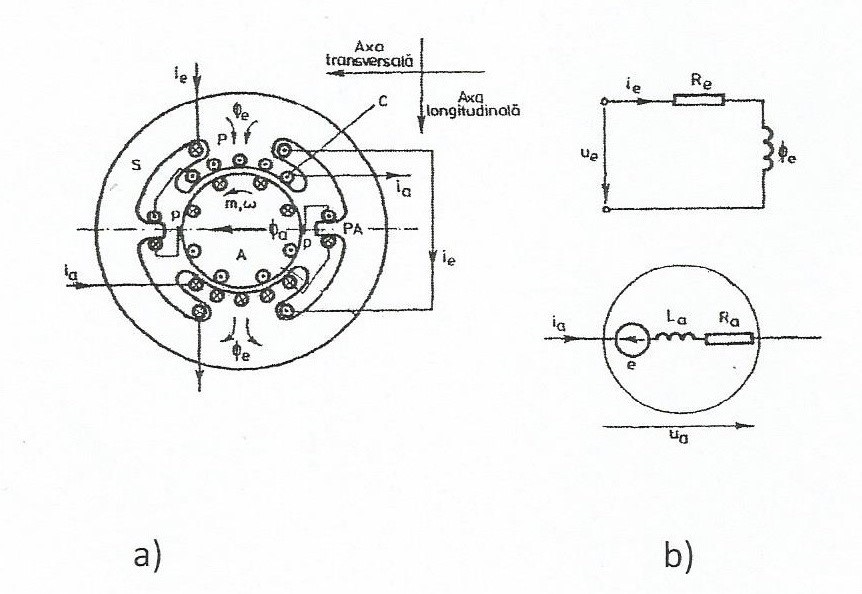
\includegraphics[width=.7\linewidth]{fig1.jpg}
	\captionof{figure}{Masina de curent continuu, cu excitatie separata}
	\label{fig:test2}
\end{figure}

Actiunea inductiva a indusului poate fi reprezentata printr-o inductivitate concentrata La. Deoarece infasurarea de compensatie si infasurarea polilor auxiliari se gasesc de asemenea in axa periilor (transversala) actiunea lor se posta lua in considerare prin La.

\section{Motorul de curent continuu cu excitatie separata \\
	Ecuatii diferentiale si schema bloc}
Schema echivalenta a motorului de curent continuu cu excitatie separata (independenta), care a fost deja reprezentata in figura 1.b, se modifica in sensul ca parametrii concentrati Ra si La se reprezinta in afara indusului (figura 2)
\begin{figure}[H]
	\centering
	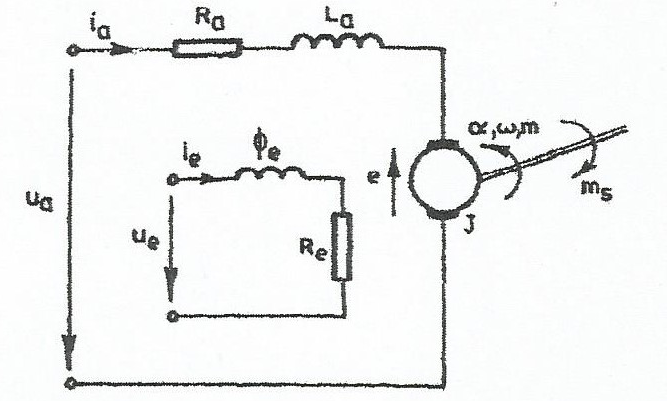
\includegraphics[width=.5\linewidth]{fig2.png}
	\captionof{figure}{Schema echivalenta a motorului de curent continuu cu excitatie separata}
	\label{fig:test2}
\end{figure}

Ca marimi de intrare actioneaza tensiunea aplicata indusului ua, tensiunea aplicata circuitului de excitatie ue si cuplul de sarcina ms.Φe este fluxul de excitatie, m este cuplul electromagnetic al motorului , iar J momentul de inertie a maselor cu miscare de rotatie. 
Aplicand teorema a doua a lui Kirchhoff circuitului indusului rezulta:
\begin{align}
u_a=e+R_ii_a+L_a\frac{di_a}{dt}
\end{align}
unde s-a neglijat caderea de tensiune la periile masinii, care depinde neliniar de curentul prin indus.

In acelasi mod, pentru circuitul de excitatie se obtine:
\begin{align}
u_e=R_ei_e+\frac{d\Phi_e}{dt}
\end{align}
Tensiunea electromotoare indusa prin rotatie va fi:
\begin{align}
e=k\Phi_e\omega, cu\ k = \frac{pN}{2\pi a}
\end{align}
unde:
\begin{enumerate}[label=$\bullet$]
	\item N - numarul de conductoare activa a infasurarii indusului;
	\item p - numarul de perechi de poli; 
	\item a - numarul de perechi de cai de curent ale infasurarii indusului;
	\item $\omega$ - viteza unghiulara a indusului (rotorului)  
\end{enumerate}
Cuplul electromagnetic exercitat asupra rotorului motorului este:
\begin{align}
m=k\Phi_ei_a
\end{align}
Ecuatia de miscare se poate scrie sub forma:
\begin{align}
m-m_s=J\frac{d\omega}{dt}
\end{align}
Ecuatia vitezei unghiulare este:
\begin{align}
\omega=\frac{d\alpha}{dt}
\end{align}
Ecuatia (1) se poate pune sub forma:
\begin{align}
T_a\frac{di_a}{dt}+i_a=\frac{1}{R_a}(u_a-e)
\end{align}
Unde $T_a=L_a/R_a$  este constanta de timp a circuitului indusului.
Ecuatia (2) scrisa sub forma:
\begin{align}
\frac{d\Phi_e}{dt}=u_e-R_ei_e
\end{align}
reprezinta ecuatia diferentiala a unui element de integrare (integrator).
\begin{figure}[H]
	\centering
	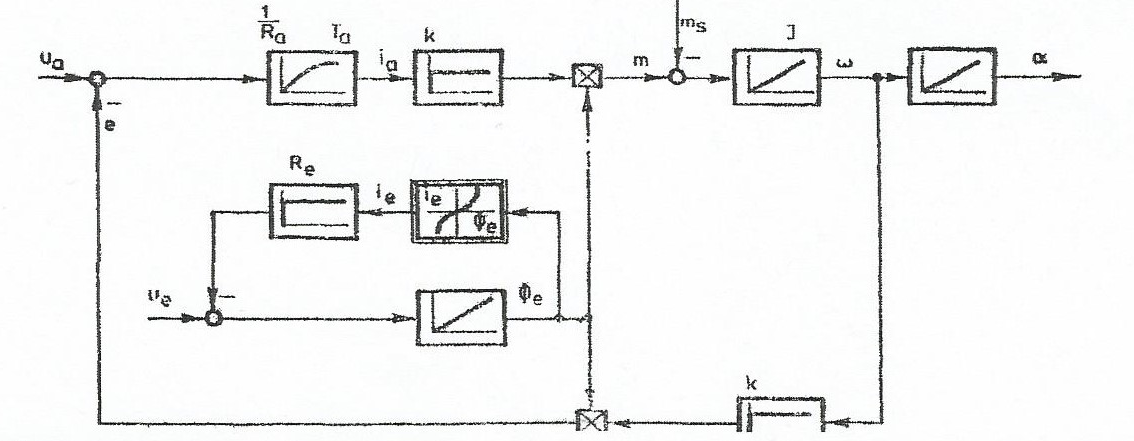
\includegraphics[width=.8\linewidth]{fig4.png}
	\captionof{figure}{Schema bloc a motorului de curent continuu cu excitatie separata (marimi absolute).}
	\label{fig:test2}
\end{figure}
Ecuatiile (7), (8), (3), (4), (6) descriu comportarea dinamica a motorului de curent continuu cu excitatie separata. Schema structu ru la sa u sche ma bloc corespunzatoare acestor ecuatii diferentialee cuplate este ilustrata in Fig. 3.

Marimile variabile care apar in schema bloc din figura 3 au diferite dimensiuni. Pastrarea neschimbata a acestor marimi ar complica calculul prin relatii dimensionale complicate. Din aceasta cauza se obisnuieste ca toate marimile sa se raporteze, adica sa devina marimi adimensionale. Se ajunge astfel la sistem de unitati relative care usureaza calculele, in special cele efectuate pe calculator.
\begin{figure}[H]
	\centering
	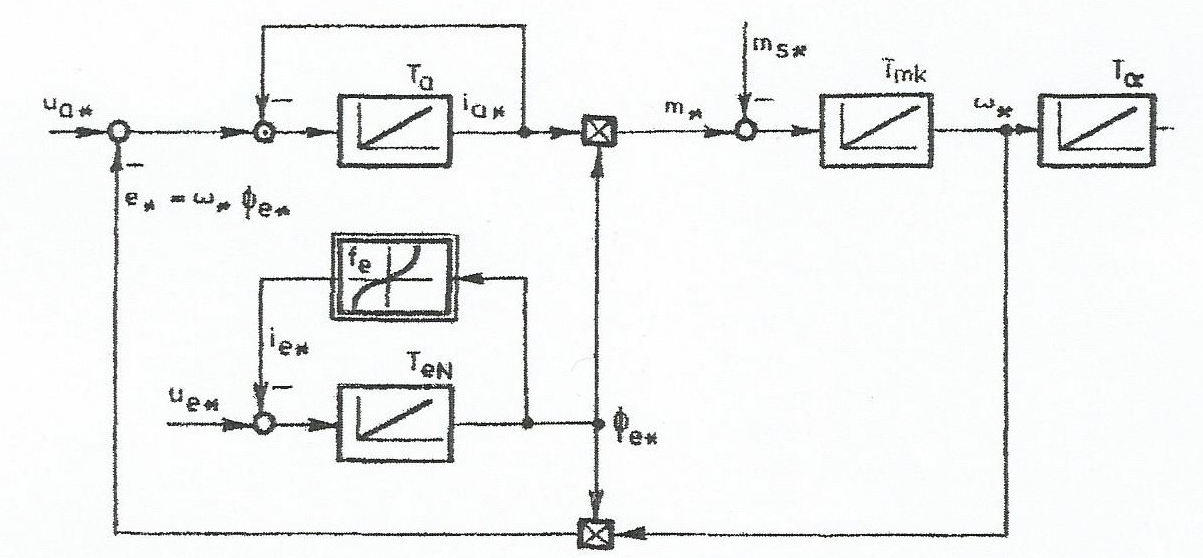
\includegraphics[width=.8\linewidth]{fig5.png}
	\captionof{figure}{Schema bloc a motorului de curent continuu cu excitatie separata (marimi relative)}
	\label{fig:test2}
\end{figure}
\section{Caracteristici mecanice stationare la comanda pe indus}
La comanda pe indus fluxul de excitatie se mentine constant, la valoarea nominala $\Phi_e=\Phi_{eN}$ si se modifica tensiunea de alimentare $u_a$;

Pentru $\Phi_e=\Phi_{eN}\frac{\Phi_{e}}{\Phi_{en}}$ dispar astfel ambele semne de multiplicare din schema bloc.
\begin{center}
	$\omega*=u_{a^*}-m_{s^*}$\\
	$i_{a^*}=m_{s^*}$
\end{center}
Caracteristicile mecanice $W* (m_{s^*})$ reprezinta o familie de drepte, parelele cu 
caracteriastica mecanica naturala $u_{a^*}=\frac{U_{aN}}{U_a}=1$ avand drept parametru $u_{a^*}=\frac{U_{aN}}{U_a}$

Caracteristicile sunt valabile in toate cele patru cadrane, deci exista posibilitatea unei reversari continue a turatiei si cuplului. Caracteristicile mecanice obtinute prin variatia tensiunii de alimentare se numesc carecteristici mecanice artificiale de tensiune. Deoarece tensiunea aplicata indusului u, este raportata la valoarea sa nominala, ne intereseaza numai domeniul $-1 \leq \frac{u_a}{u_{aN}} \leq 1$; la depasirea importanta a acestui domeniu se inrautateste 
comutatia (apar mai intai scantei la perii si apoi, posibil, foc la colector). 

Curentul prin indus (figura 5.b) este proportional cu cuplul, iar tensiunea indusului nu are nici o influenta. Cuplul este raportat la cuplul de pornire pe caracteristica mecanica naturala $m_a$ (la motoarele mari $m_a = (8 ... 10)mN)$. De aceea domeniul de functionare normal este $-0.2 \leq \frac{m}{m_0}\leq 0.2$.
\begin{figure}[H]
	\centering
	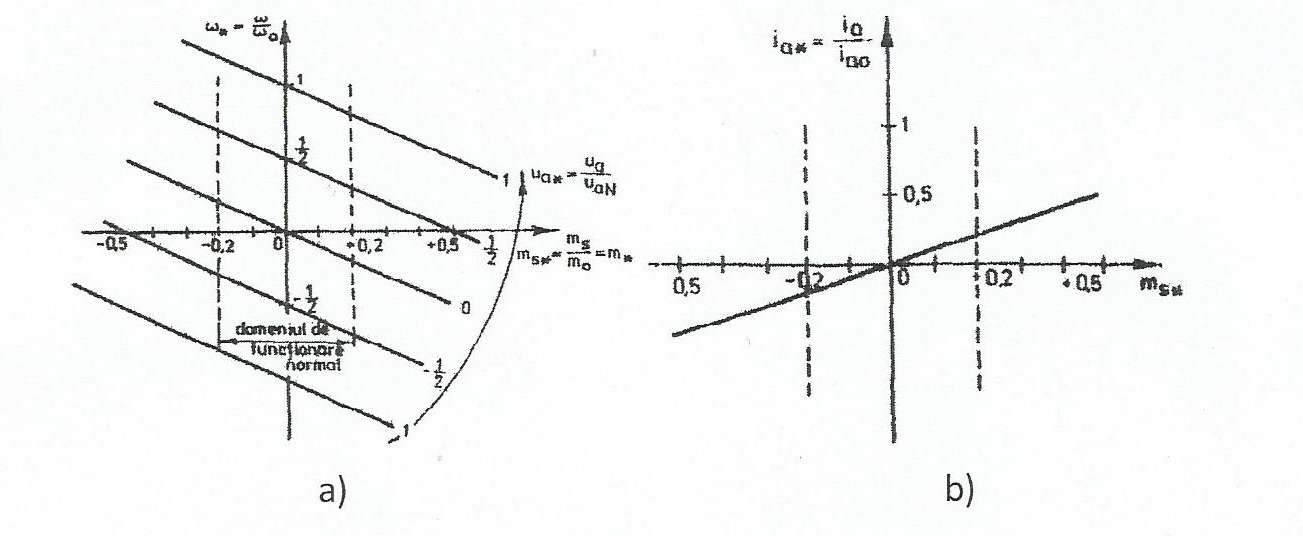
\includegraphics[width=.8\linewidth]{fig6.png}
	\captionof{figure}{Comanda pe indus a) caracteristici mecanice artificiale de tensiune b) caracteristica $i_{a^*}(m_{s^*})$}
	\label{fig:test2}
\end{figure}
In afara acestui domeniu, datorita reactiei indusului $\Phi_{e}(I_a)$, caracteristicile mecanice prezentate sunt numai partial valabile; de asemenea apar probleme de comutatie. 

Deoarece cuplul electromagnetic m respectiv cuplul de sarcina ma este raportat la valoarea cuplului de pornire, pe caracteristica mecanica naturala mo caracteristicile mecanice stationare la comanda pe indus (figura 5.a) apar mai inclinate decat cele reprezentate in marimi absolute si intalnite frecvent in lucrari de specialitate.

La flux de excitatie constant $\Phi_{e}=\Phi_{eN}$ modificarea tensiunii indusului produce o deplasare paralela a caracteristicilor mecanice in timp ce caracteristica curent-cuplu ramane constanta. Acest lucru apare deosebit de avantajos la actionarile electrice regla bile, deoarece parametrii circuitului de reglare ramain neschimbati; avem de-a face cu un element liniar. 
\section{Reglarea turatiei motoarelor de curent continuu}
In practica, alegerea unei actionari de curent continuu este determinata in mod obisnuit de posibilitatea obtinerii unui domeniu larg de variatie a turatiei, domeniu impus de procesul tehnologic. Pentru a se obtine insa comportarea de functionare dorita, la perturbatii ale retelei. de alimentare si ale sarcinii mecanice, actionarea trebuie sa fie automatizata. 

Pe de alta parte, indusul motoarelor mari prezinta o rezistenta mica si in momentul pornirii la tensiunea nominala rezulta prin indus un curent foarte mare. In functionarea stationara nu se intalneste asemenea situatie, deoarece curentul este determinat de diferenta dintre tensiunea aplicata indusului si. tensiunea electromotoare indusa. In regim nestationar este posibil ca, datorita unei schimbari prea rapide a tensiunii sau turatiei, sa apara un curent nepermis de mare. De aceea, pentru protejarea motorului, a sursei de alimentare, si a sarcinii mecanice se prevede o limitare rapida a curentului prin indus si deci a cuplului electromagnetic dezvoltat de motor.
\begin{figure}[H]
	\centering
	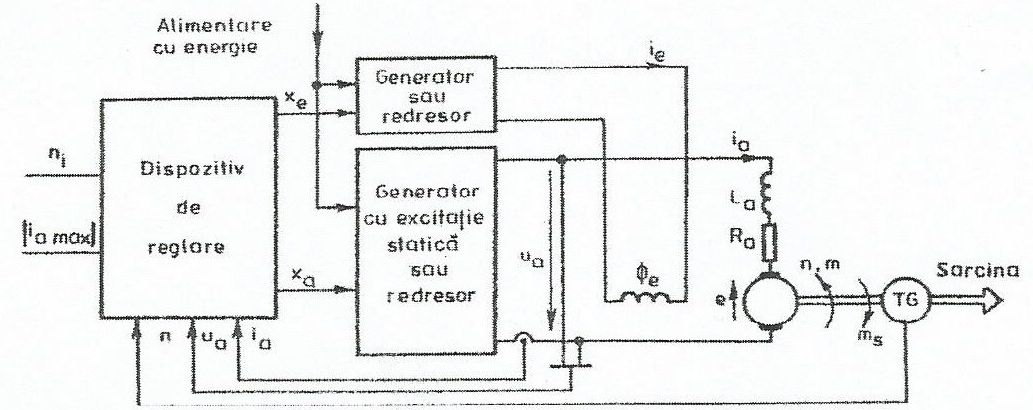
\includegraphics[width=.8\linewidth]{fig7.png}
	\captionof{figure}{Schema de principiu a unei actionari de curent continuu reglabile}
	\label{fig:test2}
\end{figure}
\section{Reglarea turatiei prin comanda pe indus}
Pentru a se micsora supracurentul prin indus si pentru a proteja motorul, fluxul de excitatie trebuie mentinut la valoarea nominala. 

In figura 7 s-a reprezentat circuitul indusului motorului si sursa de alimentare a indusului (elementul de executie). S-a notat cu ea tensiunea sursei de alimentare a indusului, comandata prin. xa, tensiune care, datorita impedantei interne (R, LJ, nu corespunde cu tensiunea u, aplicata la bornele motorului. Impedanta interna a elementului de executie trebuie luata de asemenea in considerare la definirea marimilor de referinta.
\begin{figure}[H]
	\centering
	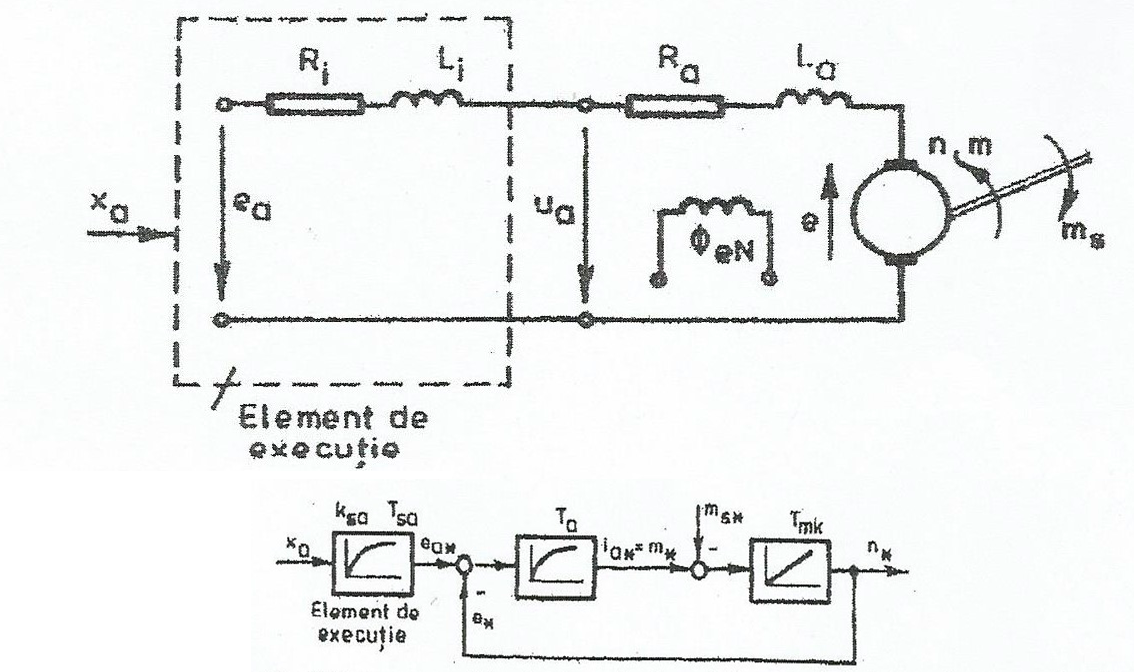
\includegraphics[width=.8\linewidth]{fig8_fin.png}
	\captionof{figure}{Schema echivalenta a indusului motorului si a elementului de executie}
	\label{fig:test2}
\end{figure}
\begin{center}
	$i_a=\frac{u_{aN}}{R_a+R_i}$ \ 	$T_a=\frac{L_a+L_i}{R_a+R_i}$
\end{center}
\begin{figure}[H]
	\centering
	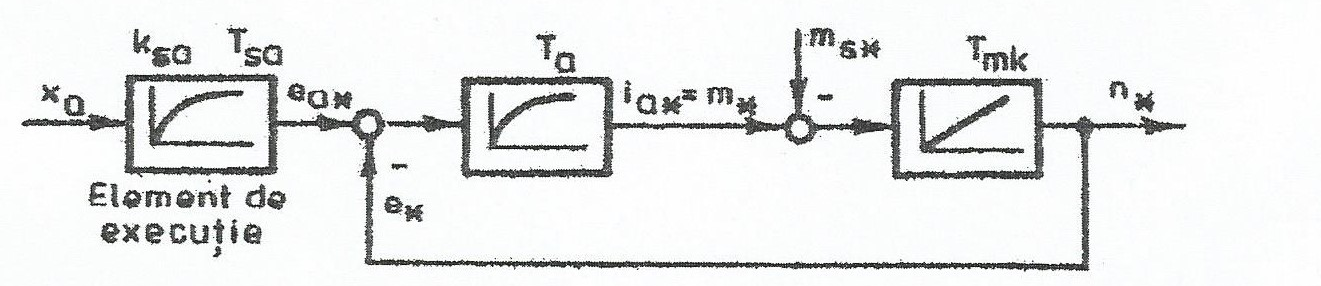
\includegraphics[width=.8\linewidth]{fig9.png}
	\captionof{figure}{Schema bloc a sistemului motor de curent continuu cu excitatie separata}
	\label{fig:test2}
\end{figure}
Pentru sursa de tensiune comandata a indusului s-a considerat un element inertial de ordinul intai (cu amplificarea ksa si constanta de timp TsJ. Valoarea constantei de timp Tsa la un redresor comandat are valoarea de (1. .. 5)ms. Constanta de timp a indusului Ta are inmod obisnuit valori cuprinse intre 10 si 100 ms; ea este determinata de impedanta circuitului indusului considerand o eventuala bobina de netezire, care la alimentarea de la redresoare este necesara pentru micsorarea ondulatiei curentului. 

Constanta, de timp Tmk se refera la momentul de inertie total al actionarii raportat la arborele motorului; ea poate varia de la ordinul milisecundelor la cateva secunde. 

Pentru reglarea turatiei cu limitarea curentului prin indus, cel mai potrivit principiu de reglare este procedeul reglarii in cascada. Reglarea in cascada are cateva insusiri importante: 
\begin{enumerate}[label=$\bullet$]
	\item permite, pe langa reglarea marimii principale (in cazul de fata turatia), limitarea marimilor auxiliare (de exemplu curentul prin indus); 
	\item fractioneaza functia de transfer a elementului de executie si procesului in portiuni, astfel incat fiecarui regulator i se repartizeaza una sau cel mult doua constante de timp importante, ceea ce face ca optimizarea se se poata realiza un regulator PID sau cu variante mai simple ale acestuia; 
	\item permite o simetrizare a operatiilor de acordare optimala a regulatoarelor 
\end{enumerate}
Pentru schema bloc a motorului se pot scrie ecuatiile:
\begin{align}
T_a\frac{di_{a^*}}{dt}+i_{a^*}=e_{a^*}-e_*
\end{align}
\begin{align}
e_*=n_*
\end{align}
\begin{align}
T_{mk}\frac{dn_{*}}{dt}=m_{*}-m_{s^*}
\end{align}
\begin{align}
i_{a^*}=m_*
\end{align}
Pe baza ecuatii lor de mai sus cu notatiile: $Ea(s) = L{ea*}; N(s) = L{n*}$ rezulta schema bloc a motorului reprezentata in figura 9.
Utilizand calculul operational ecuatiile (9) ... (12) devin:
\begin{align}
I_a(s)(a+sT_a)=E_a(s)-E(s)
\end{align}
\begin{align}
E(s)=N(s)
\end{align}
\begin{align}
sT_{mk}N(s)=M(s)-M_s(s)
\end{align}
\begin{align}
I_a(s)=M(s)
\end{align}
\begin{figure}[H]
	\centering
	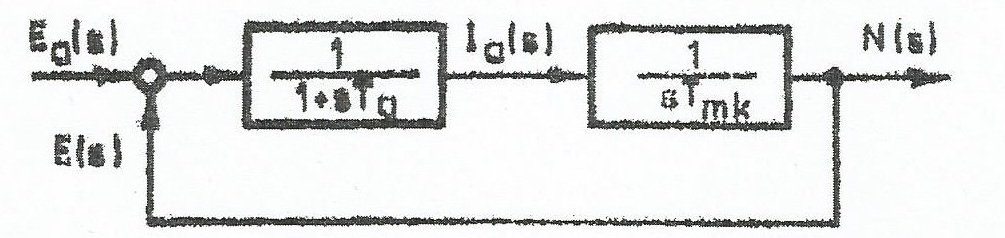
\includegraphics[width=.5\linewidth]{fig10.png}
	\captionof{figure}{Schema in lant a motorului de curent continuu cu excitatie separata}
	\label{fig:test2}
\end{figure}
Conform figurii 9 functiile de transfer pe parti sunt:
\begin{align}
\frac{I_a(s)}{E_a(s)}=\frac{\frac{1}{1+sT_a}}{1+\frac{1}{sT_a}+\frac{1}{sT_{mk}}}=\frac{sT_{mk}}{1+sT_{mk}+s^2T_aT_{mk}}
\end{align}
\begin{align}
\frac{N(s)}{I_a(s)}=\frac{1}{sT_{mk}}
\end{align}
Din relatiile (13) ... (16) rezulta:
\begin{align}
X_i(s)=E_a(s)+\frac{M_s(s)}{sT_{mk}}=\frac{1+sT_{mk}+s^2T_aT_{mk}}{sT_{mk}}I_a(s)
\end{align}
Schema bloc in lant corespunzatoare ecuatiei (12) este reprezentata in figura 10. 
Pe baza acestor rezultate, trecand din nou la reprezentarea prin functii tranzitorii, rezulta schema bloc a sistemului motor - element de executie (figura 11). In aceasta situatie reactia din bucla (figura 8) dispare. Se observa ca, cuplul de sarcina m.actioneaza in doua locuri. Marimile care nu au fost marcate nu au nici un sens fizic. Partea de reglare cuprinsa intre ea* si ia* (figura 12) poate fi descrisa prin functia de transfer: 
\begin{center}
$\frac{I_a(s)}{E_a(s)}=\frac{sT_{mk}}{1+sT_{mk}+s^2T_aT_{mk}}$
\end{center}
Trebuie observat ca efectul de diferentiere este urmarea compensarilor tensiunilor ea si e la mersul in got. Polinomul de la numitor poate prezenta poli reali sau complecsi conjugati.
\begin{figure}[H]
	\centering
	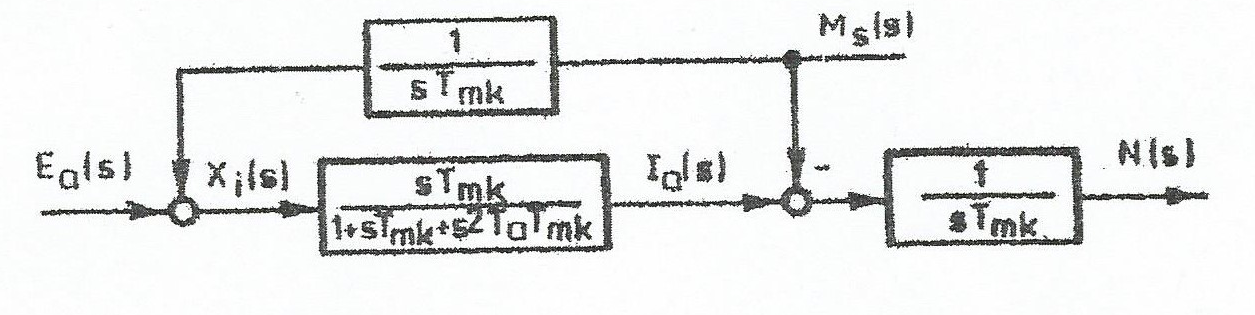
\includegraphics[width=.7\linewidth]{fig11.png}
	\captionof{figure}{Schema in lant a motorului de c.c. cu excitatie separata pentru $M_s(s)\neq0$}
	\label{fig:test2}
\end{figure}
Potrivit principiului reglarii in cascada, marimea care trebuie limitata este mentinuta sub control printr-un circuit de reglare interior. In. figura 11 este prezentata dispunerea acestui circuit. Valoarea reala a curentului este sesizata printr-un traductor si este supusa unei neteziri. In cele mai multe cazuri o constanta de timp $T_t$ de 5 ms este suficienta.
\begin{figure}[H]
	\centering
	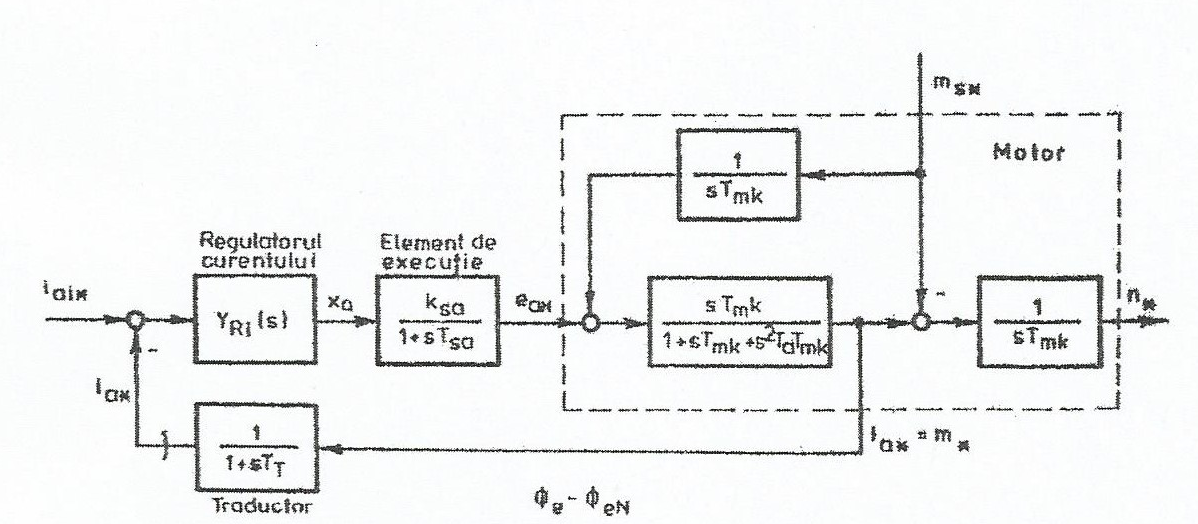
\includegraphics[width=.9\linewidth]{fig12.png}
	\captionof{figure}{Dispunerea circuitului de reglare a curentului la un sistem de actionare motor de c.c. cu excitatie separata - element de executie.}
	\label{fig:test2}
\end{figure}
Daca se foloseste un redresor comandat ca element de executie, ca regulator al curentului este suficient un regulator PI. 
Schemele de reglare a actionarilor electrice trebuie sa permita si pornirea automata a motorului. Pentru a alimenta cu curent constant un motor care porneste in gol - din cauza turatiei care creste liniar in timp - este necesara o tensiune crescatoare. Dar o asemenea marime de iesire variabila in timp pretinde la un regulator simplu integral o abatere de reglare. In cazurile practice nu deranjeaza faptul ca circuitul de reglare a curentului prezinta o eroare de reglare interior. 

Dimensionarea regulatorului curentului se realizeaza conform procedeelor obisnuite din tehnica reglarii. Pentru acordarea optima a regulatorului curentului se utilizeaza varianta Kessler a criteriului modulului.

Circuitul de reglare a curentului, astfel dimensionat, se introduce (figura 12) in circuitul supraordonat de reglare a turatiei; in ipoteza unei bune amortizari in circuitul de reglare a curentului sa se aproximeze printr-un element inertial de ordinul intai avand constanta de timp Ti si factorul de amplificare k, (figura 12).

Constanta de timp $T_i$ va fi:
\begin{align}
T_i=2T_{\Sigma i}=2(T_{sa}+T_\gamma)
\end{align}
Iar factorul de amplificare:
\begin{align}
k_i=\frac{i_{a\max}}{U_{sat}}
\end{align}
Unde:
\begin{enumerate}[label=$\bullet$]
	\item $I_{a\max}$ - valoarea limita a curentului prin indus 
	\item $U_{sat}$ - tensiunea de saturatie a regulatorului precedent (regulatorul turatiei) 
\end{enumerate}
Pentru circuitul de reglare a turatiei se ia de asemenea in considerare un regulator PI. Rezulta astfel functia de transfer a circuitului deschis (figura 12).
\begin{figure}[H]
	\centering
	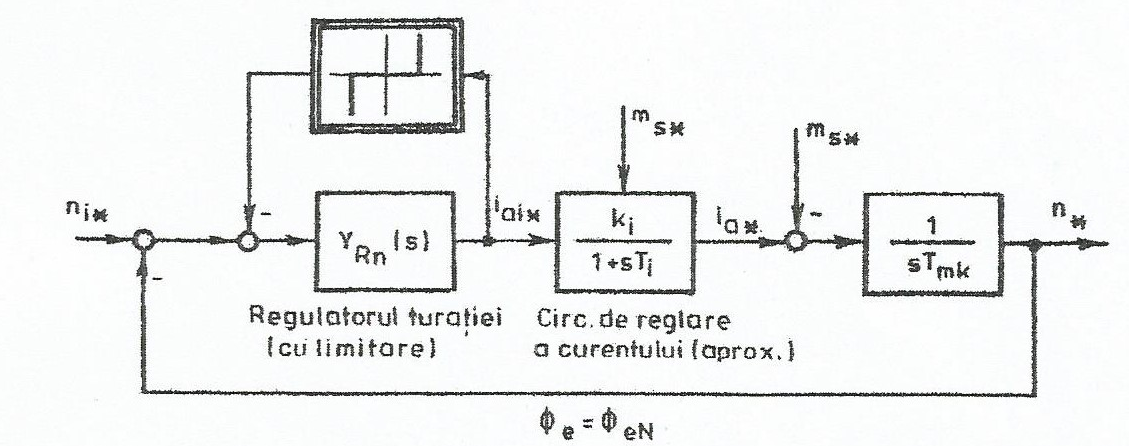
\includegraphics[width=.9\linewidth]{fig13.png}
	\captionof{figure}{Dispunerea circuitului de reglare a turatiei la un sistem de actionare motor e.e. cu excitatie separata- element de executie}
	\label{fig:test2}
\end{figure}

\begin{align}
Y_n(s)\equiv k_Rn \frac{1+sT_{in}}{sT_{in}} \frac{k_i}{1+sT_i} \frac{1}{sT_{mk}}
\end{align}

Acordarea optima a regulatorului, adica determinarea parametrilor $k_{Rn}$ si $T_{in}$, se efectueaza conform criteriului simetriei. In figura 12 regulatorul turatie, este prevazut cu o reactie neliniara; aceasta impiedica cresterea valorii impuse a curentului Iai* peste valoarea limita Tia max*. In acest fel se protejeaza instalatia de alimentare impotriva supraincarcarii. 
Limitarea valorii impuse a curentului permite de asemenea sa se dea o variatie oarecare valorii impuse a turatiei.

\newpage
\section{Breviar de calcul}
Curentul nominal rotoric:

\begin{align*} 
 I_n=\frac{P_N}{n\times U_n}=\frac{3.7 \ast 10^3}{0.77 \times 190}=25.29A
 \end{align*}
 Curentul maxim: $I_{max}=1.9\ast I_N=1.9\times 25.29 = 48.05 A$
 
 Daca se admite caderea de tensiune pe bobina de filtraj a circuitului cu redresoare la trecerea curentului nominal, estimat la 2.5\% din tensiunea nominala, rezulta rezistenta:
 \begin{align*} 
 R_b=\frac{0.025\times U_N}{I_N}=\frac{0.025\times 190}{25.29}=0.18\Omega
 \end{align*}
 Tensiunea maxima la iesirea din puntea redresoare va fi:
 \begin{align*} 
 U_{d0}=U_N+R_b\ast I_N= 190+0.18\times 25.29=194.55 V
 \end{align*}
 Tensiunea de linie din secundarul transformatorului care alimenteaza puntea redresoare va fi:
 \begin{align*} 
U_{l2}=\frac{U_{d0}}{1.35}=144.11 V
 \end{align*}
Se mentioneaza de asemenea neglijarea caderilor de tensiune pe tiristoare.

Rezistenta rotorica poate fi apreciata aproximativ, observand ca puterea de pierderi nominale in cuprul rotoric reprezinta circa jumatate din pierderile nominale totale, adica:
\begin{align*} 
P_{Cu2}=R_aI_{aN}^2\approx\frac{U_NI_N-P_N}{2}W
\end{align*}
\begin{align*}
R_a\approx\frac{\frac{U_NI_N-P_N}{2}}{I_{aN}^2}=\frac{552.55}{639.58}=0.86\Omega
\end{align*}
\subsection{Dimensionarea tiristoarelor}
Tensiunea inversa de varf, la care va fi solicitat tiristorul va fi :
\begin{align*}
U_i=\sqrt{2}U_{l2}=203.92
\end{align*}
Valoarea nominala a curentului printr-un tiristor:
\begin{align*}
I_{nT}=I_N=25.29A
\end{align*}
Cand prin motor va trece curentul maxim, valoarea maxima a curentului prin tiristor va fi :
\begin{align*}
I_{nTmax}=2*I_N=50.58A
\end{align*}
Pentru alegerea tiristoarelor se mai au in vedere:
\begin{enumerate}[label=$\bullet$]
	\item un coeficient de siguranta de aprox. 2, al tensiunii maxime de varf admise de tiristor, fata de tensiunea de varf U;
	\item temperatura a aerului de racire de \ang{40}C
\end{enumerate}
In functie de acestea se aleg din catalogul de tiristoare, tiristoare tip KIT 2848 cu racire pe radiator. Acest tiristor admite o tensiune inversa de varf periodica de 1000V si un curent nominal de 50A.
Coeficientul de siguranta al tensiunii inverse va fi:
\begin{align*}
C_u=\frac{U_{iv}}{U_i}=\frac{1000}{203.92}=4.9
\end{align*}
\subsection{Dimensionarea bobinei de filtrare}
Inductanta bobinei de filtraj se alege astfel incat sa nu existe regim de curent interupt la unghiuri de comanda intre \ang{0} si \ang{90}, in regim de mers in gol.

Se apreciaza curentul de mers in gol la valoarea:
\begin{align*}
I_0=0.05I_N=1.26A
\end{align*}
Componenta alternativa fundamentala a tensiunii redresate (de frecventa 300Hz fiind redresare trifazata in punte) la $\alpha=\ang{90}$ este:
\begin{align*}
U_{300}=0.33U_{d0}=0.33\times 194.55=64.18V
\end{align*}
Frecventa redresarii in punte:
\begin{align*}
f_p=6\times f=300Hz
\end{align*}
Pentru a evita regimul de curent intrerupt trebuie ca valoarea maxima a componentei de 300Hz a curentului $I_{300}$ sa fie mai mica decat curentul de mers in gol:
\begin{align*}
\sqrt{2}I_{300}=0.05I_N=\frac{U_{300}\sqrt{2}}{2\pi300L_b}
\end{align*}
deci:
\begin{align*}
L_b\geq\frac{U_{300}\sqrt{2}}{2\pi300I_0}=\frac{90.76}{2375.04}=38mH
\end{align*}
\subsection{Calculul schemei de reglare}
Schema funcţională a sistemului de reglare automată în care se evidenţiează elementul de execuţie şi traductorul de măsură e prezentat în figura, 13:
\begin{figure}[H]
	\centering
	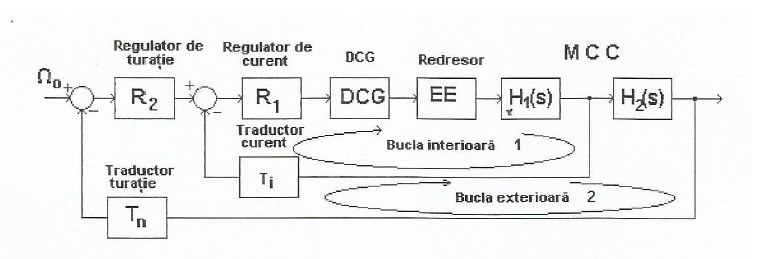
\includegraphics[width=.9\linewidth]{fig14.png}
	\captionof{figure}{schema functionala}
	\label{fig:test2}
\end{figure}
Schema de functionare evidentiează două bucle:
\begin{enumerate}
	\item Bucla interioară în care mărimea de reacţie este curentul rotoric al motorului.
	\item Bucla exterioară în care mărimea de reacţie este turaţia motorului.
\end{enumerate}
In aceste figuri s-a notat:
\begin{enumerate}[label=$\bullet$]
	\item $T_i$ traductorul de curent rotoric cu funcţia de transfer $HT_i(s)$
	
	 $T_n$ traductorul de turatie cu funcţia de transfer $HT_n(s)$
	\item DCG dispozitiv comandă pe grilă ( porţi tiristoare) cu funcţia de transfer $H DCG (s)$. Redresor comandat cu tiristoare cu funcţia de transfer $H_p(s)$ este partea principală al elementului de execuţie.
	\item $R_1$ regulator automat de curent din bucla interioară cu funcţia de transfer $HR_1(s)$
	
	 $R_2$ regulator de turatie din bucla exterioara cu funcţia de transfer $HR_2(s)$
	\item $H_1' (s)$ funcţia de transfer a motorului de curent continuu (obiectul condus din bucla interioară).
	\item $H_2 (s)$ funcţia de transfer a motorului de curent continuu din bucla exterioară.
\end{enumerate}
Alegerea aparaturii

Curentul motorului este masurat intr-un amplificator pentru traductoare de 10V/100mV. Pentru obtinerea tensiunii de circa 100mV se foloseste un sunt de 75mV/100A.

Turatia se masoara cu ajutorul unui tahogenerator de curent continuu de 100V/1000rot/min.

\subsection{Bucla de reglare a curentului}
Din cele expuse anterior si cu datele de catalog ale motorului se poate calcula inductanta indusului, conform relatiei:
\begin{align*}
L_a=\frac{5.6U_N}{npI_n}=\frac{5.6\ast190}{2500\ast 1\ast 25.29}=16mH
\end{align*}
Constanta de timp a indusului se calculeaza cu formula:
\begin{align*}
T_r=\frac{L_r}{R_r}
\end{align*}
Unde:
\begin{align*}
L_r=L_a+L_b=16+38=54mH=0.054H
\end{align*}
\begin{align*}
R_r=R_a+R_b=0.18+0.86=1.04\Omega
\end{align*}
Rezulta:
\begin{align*}
T_r=\frac{0.054}{1.04}=0.051s=51 ms
\end{align*}
Functia de transfer a motorului in bucla de reglare a curentului este:
\begin{align*}
H_{m1}(s)=\frac{I_a(s)}{U_a(s)}=\frac{1}{R_r}\frac{s T_m}{1+sT_m+s^2T_mT_r}
\end{align*}
Costanta de timp electromecanica a motorului $T_m $se calculeaza cu formula:
\begin{align*}
T_m=\frac{GD^2}{375}\frac{R_r}{(K_e\varphi)(K_m\varphi)}
\end{align*}
Unde:
\begin{align*}
K_e\varphi=\frac{U_a-R_aI_N}{n}=\frac{190-0.86\times 25.29}{2500}=0.067 \frac{V}{rot/min}
\end{align*}
\begin{align*}
K_m\varphi=\frac{K_e\varphi}{1.03}=\frac{0.067}{1.03}=0.065 Kg\ast m/A
\end{align*}
Momentul de giratie raportat la arborele motorului este:
\begin{align*}
GD^2=GD_R^2+GD_s^2=4.9 Kg\ast m^2
\end{align*}
Rezulta:
\begin{align*}
T_m=\frac{4.9}{375}\frac{1.04}{0.067\times 0.065}=0.013\ast 238.8=3.104s
\end{align*}
\subsection{Puntea de tiristoare comandate}
Indusul se alimenteaza de la un convertor trifazat reversibil (bidirectional) in puntecomplet comandat.

Fiind folosita o punte trifazata de tiristoare, timpul mort al acesteia este in medie statica:
\begin{align*}
T_p=\frac{1}{2qf}
\end{align*}
unde q este numarul de pulsuri al conexiunii redresoare iar f este frecventa.
Deci:
\begin{align*}
T_p=\frac{1}{2\times 6 \times 50}=1.67ms
\end{align*}
Factorul de amplificare maxim al puntii (la $\alpha = \ang{90}$) este:
\begin{align*}
k_p=\frac{\pi U_{d0}}{180}=\frac{194.55\times 3.14}{180}=3.392 V/grad
\end{align*}
Deci functia de transfer a puntii este:
\begin{align*}
H_p(s)=k_pe^{-sT_m}
\end{align*}
Elementul cu timp mort se inlocuieste cu un element de intarziere de ordin 1 cu functia de transfer:
\begin{align*}
H_p(s)=\frac{k_p}{1+sT_p}
\end{align*}
\subsection{Dispozitiviul de comanda pe grila}
Dispozitivul de comanda pe grila este un element proportional avand factorul de amplificare cu valoarea:
\begin{align*}
k_{DCG}=\frac{\ang{180}}{16V}=11.25 grad/V
\end{align*}
A vand in vedere ca DCG este un element liniar neinertial functia sa de transfer este:
\begin{align*}
H_{DCG}(s)=11.25 grad/V
\end{align*}
\subsection{Circuitul de masurare a curentului}

\newpage
\nocite{*}
\bibliographystyle{ieeetr}
\bibliography{bibliografie}

\end{document}